\documentclass[11pt]{article}

\usepackage[margin=1in]{geometry}
\usepackage{graphicx}

\usepackage{tikz}
\usetikzlibrary{automata}
\usetikzlibrary{arrows}
\usetikzlibrary{positioning}
\usetikzlibrary{decorations.markings}
\usetikzlibrary{lindenmayersystems}



\title{Algorithmic Molecular Self-assembly of Fractals by Cotranscriptional Folding\footnote{This work is in part supported by JST Program to Disseminate Tenure-Tracking System, MEXT, Japan, No.~6F36 and by JSPS KAKENHI Grant-in-Aid for Young Scientists (A) No.~16H05854 to S.~S.}}
\author{Yusei Masuda, Shinnosuke Seki, and Yuki Ubukata}
\date{Department of Computer and Network Engineering, University of Electro-Communications}


\begin{document}

\maketitle

\thispagestyle{empty}

RNA sequences immediately start folding upon itself as they emerge from the RNA polymerase enzyme (\textit{cotranscriptional folding}). 
Geary, Rothemund, and Andersen have recently demonstrated the capability of cotranscriptional folding to manufacture an RNA molecule of an intended shape (rectangular tile) at nano-scale [Geary et al., \textit{Science}, 345(6198):799-804, 2014]. 
Using a novel computational model of cotranscriptional folding called the \textit{oritatami system} [Geary et al., Proc.~MFCS~2016, LIPIcs 58: 43:1-43:14, 2016], we shall initiate the theoretical study on algorithmic self-assembly of shapes by cotranscriptional folding. 

\begin{figure}[h]
\centering
\begin{minipage}{0.35\linewidth}
\centering
\scalebox{0.7}{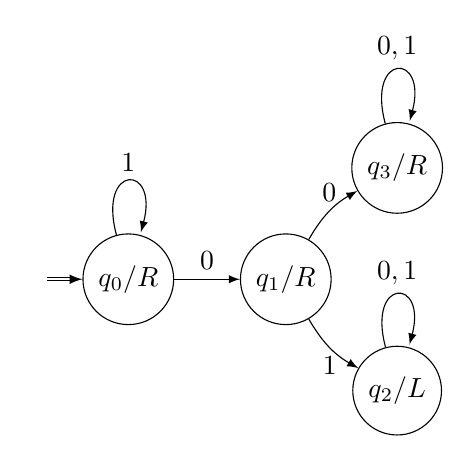
\begin{tikzpicture}[>=latex, node distance=2cm, initial text=, bend angle=15]
	\tikzstyle{every initial by arrow} = [->, double];

	\node [state, initial] (q_0)                        {$q_0/R$};
	\node [state]                     (q_1) [right of = q_0]  {$q_1/R$};
	\node [state]                     (q_2) [below right of = q_1] {$q_2/L$};
	\node [state]                     (q_3) [above right of = q_1] {$q_3/R$};

	\path [->] (q_0) edge [right] node [above]              {$0$}                 (q_1)
         		         edge [loop above] node [above]             {$1$}               ()
         			   (q_1) edge [bend left] node [above]             {$0$}                 (q_3)
         		         edge [bend right] node [below]             {$1$}              (q_2)
         			   (q_2)  edge [loop above] node [above]             {$0,1$}               ()
         			   (q_3)  edge [loop above] node [above]             {$0,1$}               ();
\end{tikzpicture}}
\end{minipage}
\begin{minipage}{0.05\linewidth}
\ \\
\end{minipage}
\begin{minipage}{0.5\linewidth}
\centering
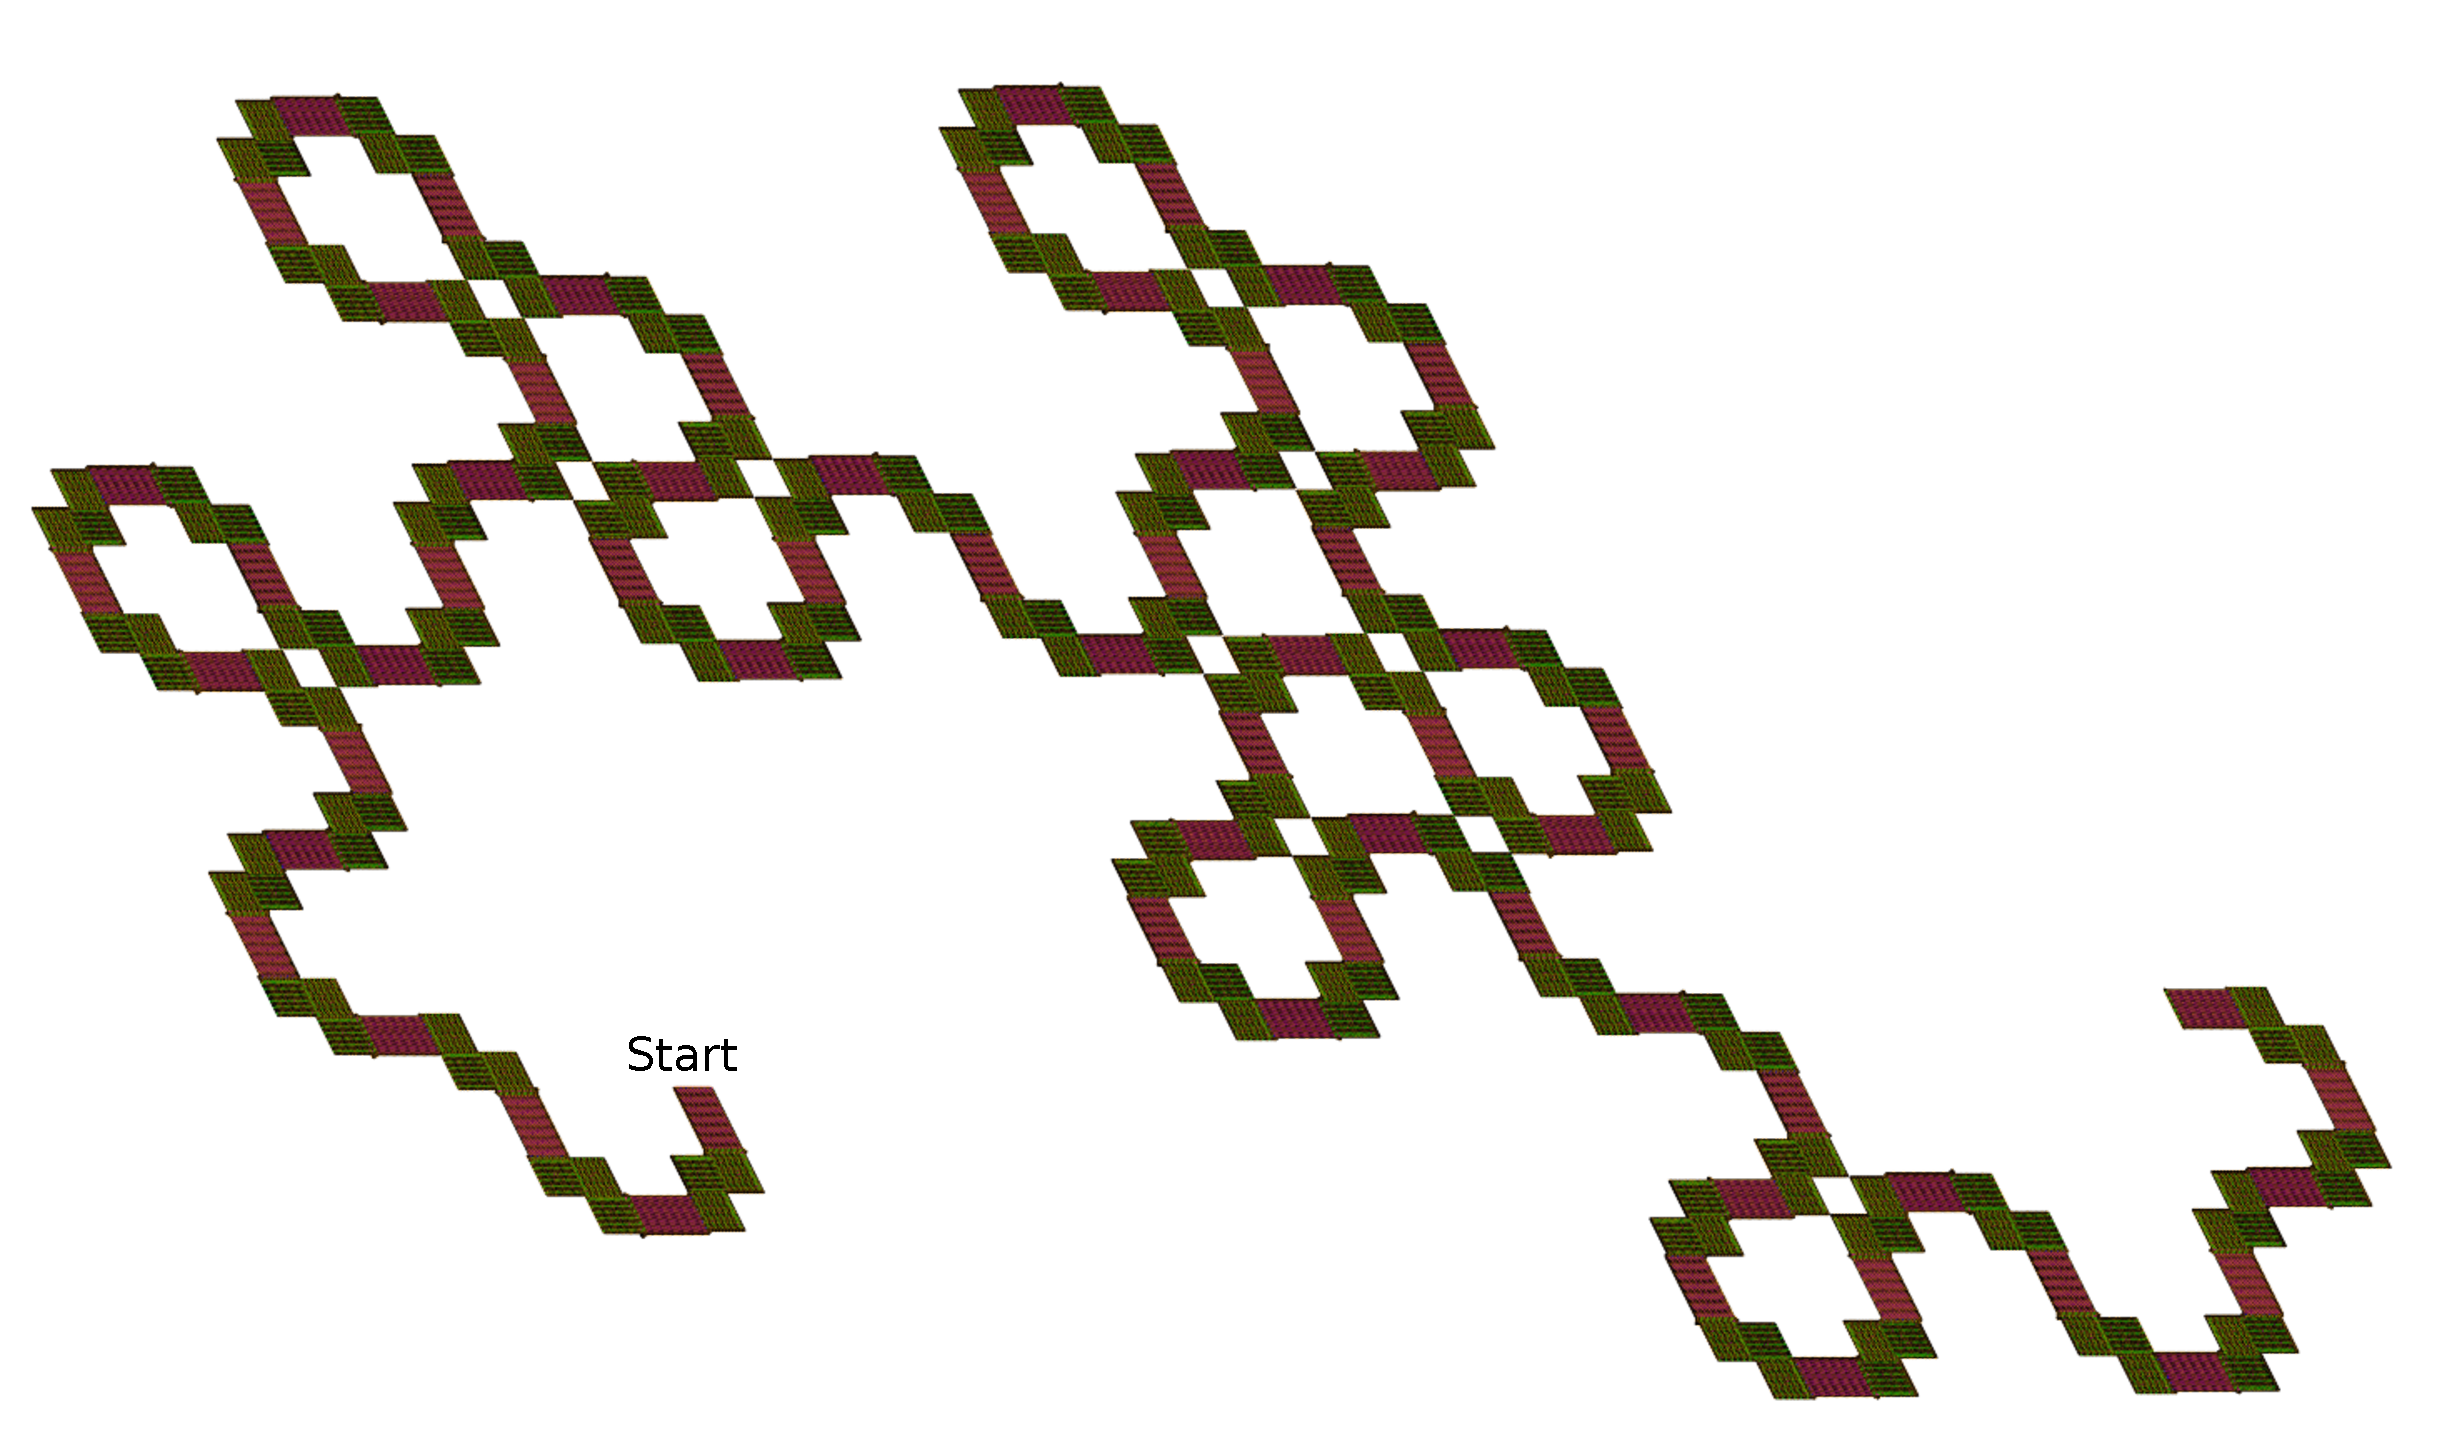
\includegraphics[width=0.9\linewidth]{6bit_heighway.pdf}
\end{minipage}
\caption{
Heighway dragon. 
(Left) A DFAO that outputs a turtle program for Heighway dragon. 
(Right) The 6th iteration of the Heighway dragon folded by the proposed oritatami system. 
}
\label{fig:heighway_dragon}
\end{figure}

Algorithms and computation are fundamental to molecular self-assembly as illustrated in their enormous success in DNA tile self-assembly. 
The Heighway dragon is a fine starting example in order to cut to the heart of algorithmic self-assembly by cotranscriptional folding because it is traversable algorithmically. 
An algorithmic way to traverse it is to feed a turtle program with the binary \textit{automatic sequence} RRLRRLLRRRLLRLL \dots as a direction to turn, whose $i$-th bit (starting from 0) can be obtained by giving a binary representation of $i$ from LSB to the DFA with output (DFAO) in Figure~\ref{fig:heighway_dragon} (Left). 
Our oritatami system combines the existing binary counter and copier modules with two modules: 
one implements the DFAO and computes the direction to turn from the current count $i$, which is propagated through a red line segment consisting of a counter and copiers; 
the other (green L-shaped block) bends the count $i$ leftward or rightward according to the direction just computed. 
The 6th iteration of the Heighway dragon, i.e., the first $2^{6}-1$ turns of it, folded by the proposed oritatami system is shown in Figure~\ref{fig:heighway_dragon} (Right). 
The system architecture is generic and works for an arbitrary finite portion of the Heighway dragon. 

\end{document}
